\documentclass[handout,nooutcomes,noauthor]{ximera}

\graphicspath{  
{./}
{./whoAreYou/}
{./drawingWithTheTurtle/}
{./bisectionMethod/}
{./circles/}
{./anglesAndRightTriangles/}
{./lawOfSines/}
{./lawOfCosines/}
{./plotter/}
{./staircases/}
{./pitch/}
{./qualityControl/}
{./symmetry/}
{./nGonBlock/}
}


%% page layout
\usepackage[cm,headings]{fullpage}
\raggedright
\setlength\headheight{13.6pt}


%% fonts
\usepackage{euler}

\usepackage{FiraMono}
\renewcommand\familydefault{\ttdefault} 
\usepackage[defaultmathsizes]{mathastext}
\usepackage[htt]{hyphenat}

\usepackage[T1]{fontenc}
\usepackage[scaled=1]{FiraSans}

%\usepackage{wedn}
\usepackage{pbsi} %% Answer font


\usepackage{cancel} %% strike through in pitch/pitch.tex


%% \usepackage{ulem} %% 
%% \renewcommand{\ULthickness}{2pt}% changes underline thickness

\tikzset{>=stealth}

\usepackage{adjustbox}

\setcounter{titlenumber}{-1}

%% journal style
\makeatletter
\newcommand\journalstyle{%
  \def\activitystyle{activity-chapter}
  \def\maketitle{%
    \addtocounter{titlenumber}{1}%
                {\flushleft\small\sffamily\bfseries\@pretitle\par\vspace{-1.5em}}%
                {\flushleft\LARGE\sffamily\bfseries\thetitlenumber\hspace{1em}\@title \par }%
                {\vskip .6em\noindent\textit\theabstract\setcounter{question}{0}\setcounter{sectiontitlenumber}{0}}%
                    \par\vspace{2em}
                    \phantomsection\addcontentsline{toc}{section}{\thetitlenumber\hspace{1em}\textbf{\@title}}%
                     }}
\makeatother



%% thm like environments
\let\question\relax
\let\endquestion\relax

\newtheoremstyle{QuestionStyle}{\topsep}{\topsep}%%% space between body and thm
		{}                      %%% Thm body font
		{}                              %%% Indent amount (empty = no indent)
		{\bfseries}            %%% Thm head font
		{)}                              %%% Punctuation after thm head
		{ }                           %%% Space after thm head
		{\thmnumber{#2}\thmnote{ \bfseries(#3)}}%%% Thm head spec
\theoremstyle{QuestionStyle}
\newtheorem{question}{}



\let\freeResponse\relax
\let\endfreeResponse\relax

%% \newtheoremstyle{ResponseStyle}{\topsep}{\topsep}%%% space between body and thm
%% 		{\wedn\bfseries}                      %%% Thm body font
%% 		{}                              %%% Indent amount (empty = no indent)
%% 		{\wedn\bfseries}            %%% Thm head font
%% 		{}                              %%% Punctuation after thm head
%% 		{3ex}                           %%% Space after thm head
%% 		{\underline{\underline{\thmname{#1}}}}%%% Thm head spec
%% \theoremstyle{ResponseStyle}

\usepackage[tikz]{mdframed}
\mdfdefinestyle{ResponseStyle}{leftmargin=1cm,linecolor=black,roundcorner=5pt,
, font=\bsifamily,}%font=\wedn\bfseries\upshape,}


\ifhandout
\NewEnviron{freeResponse}{}
\else
%\newtheorem{freeResponse}{Response:}
\newenvironment{freeResponse}{\begin{mdframed}[style=ResponseStyle]}{\end{mdframed}}
\fi



%% attempting to automate outcomes.

%% \newwrite\outcomefile
%%   \immediate\openout\outcomefile=\jobname.oc
%% \renewcommand{\outcome}[1]{\edef\theoutcomes{\theoutcomes #1~}%
%% \immediate\write\outcomefile{\unexpanded{\outcome}{#1}}}

%% \newcommand{\outcomelist}{\begin{itemize}\theoutcomes\end{itemize}}

%% \NewEnviron{listOutcomes}{\small\sffamily
%% After answering the following questions, students should be able to:
%% \begin{itemize}
%% \BODY
%% \end{itemize}
%% }
\usepackage[tikz]{mdframed}
\mdfdefinestyle{OutcomeStyle}{leftmargin=2cm,rightmargin=2cm,linecolor=black,roundcorner=5pt,
, font=\small\sffamily,}%font=\wedn\bfseries\upshape,}
\newenvironment{listOutcomes}{\begin{mdframed}[style=OutcomeStyle]After answering the following questions, students should be able to:\begin{itemize}}{\end{itemize}\end{mdframed}}



%% my commands

\newcommand{\snap}{{\bfseries\itshape\textsf{Snap!}}}
\newcommand{\flavor}{\link[\snap]{https://snap.berkeley.edu/}}
\newcommand{\mooculus}{\textsf{\textbf{MOOC}\textnormal{\textsf{ULUS}}}}


\usepackage{tkz-euclide}
\tikzstyle geometryDiagrams=[rounded corners=.5pt,ultra thick,color=black]
\colorlet{penColor}{black} % Color of a curve in a plot



\ifhandout\newcommand{\mynewpage}{\newpage}\else\newcommand{\mynewpage}{}\fi

\usepackage{fullpage}
\makeatletter
%% no number for activity
\newcommand\logostyle{%
  \def\activitystyle{activity-chapter}
  \def\maketitle{%
                {\flushleft\small\sffamily\bfseries\@pretitle\par\vspace{-1.5em}}%
                {\flushleft\LARGE\sffamily\bfseries\@title \par }%
                {\vskip .6em\noindent\textit\theabstract\setcounter{problem}{0}\setcounter{sectiontitlenumber}{0}}%
                    \par\vspace{2em}
                    \phantomsection\addcontentsline{toc}{section}{\textbf{\@title}}%
                     \setcounter{titlenumber}{0}}}
\makeatother
\newcommand{\nameblankgen}{\noindent\textbf{Name(s) (please print):}\ \hrulefill \\

\hrulefill}
\logostyle


\title{Rep-tiles}

\author{Bart Snapp}

\begin{document}
\begin{abstract}
  We will investiagte rep-tiles.
\end{abstract}
\maketitle

\noindent\textbf{Group members (please print):}\ \hrulefill \\

\hrulefill
A \textbf{rep-tile}\index{rep-tile} is a polygon where several copies of
a given rep-tile fit together to make a larger, similar, version of
itself. If $2$ copies are used, we call it a \textit{rep-2-tile}, if
$3$ copies are used, we call it a \textit{rep-3-tile}, and if $n$ copies
are used, we call it a \textit{rep-n-tile}.


\begin{problem}
With a separate sheet of paper, draw and cut out:
\begin{enumerate}
\item An isosceles right triangle whose sides have lengths $1''$, $1''$, and $\sqrt{2}''$.
\item A rectangle whose sides have lengths $1''$ and $\sqrt{2}''$.
\end{enumerate}
Working with a partner, show that each of these polygons is a rep-2-tile.
\end{problem}

\begin{problem}
For each rep-tile above, compute the perimeter and area. In each case,
how does this relate to the perimeter and area of the larger polygon?
\end{problem}


\begin{problem}
With a fresh sheet of paper, start a table:
\begin{center}
\begin{tabular}{c|c|c}
rep-$n$-tile & $\dfrac{\text{new perimeter}}{\text{old perimeter}}$ & $\dfrac{\text{new area}}{\text{old area}}$  \\
\hline\hline
 2 & $\vdots$  &  $\vdots$  \\ 
3 & $\vdots$  &  $\vdots$  \\ 
\end{tabular}
\end{center}
\end{problem}


\begin{problem}
Geometry Giorgio suggests that a rectangle whose sides have lengths
$1''$ and $4''$ is also a rep-2-tile. Is he right? If you should
happen to search the internet for other examples of rep-2-tiles, you
might find a surprise.
\end{problem}


\begin{problem}
With a separate sheet of paper, draw and cut-out:
\begin{enumerate}
\item A 30-60-90 right triangle whose shortest side has length $1''$.
\item A rectangle whose sides have lengths $1''$ and $\sqrt{3}''$.
\end{enumerate}
Working with a partner, show that each of these polygons is a rep-3-tile.
\end{problem}

\begin{problem}
For each rep-tile above, compute the perimeter and area. In each case,
how does this relate to the perimeter and area of the larger polygon?
Add this information to your table.
\end{problem}


\begin{problem}
Explain why every triangle and every parallelogram is a
rep-4-tile. Give an example of each, and compute the perimeter and
area. In both cases, compare the perimeter and area to that of the
larger polygons.
\end{problem}


\break

\begin{problem}
With a separate sheet of graph paper, draw and cut out the following polygons:
\[
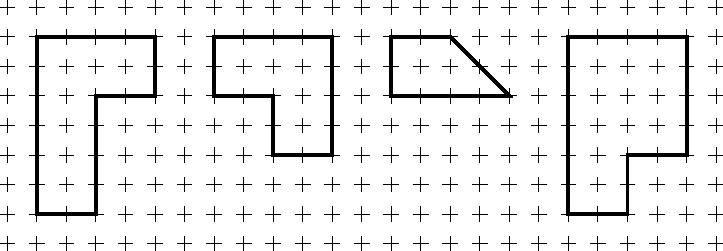
\includegraphics{rep-4-tile1.pdf}
\]
Working with a partner, show that each of these polygons is a rep-4-tile.
\end{problem}

\begin{problem}
For each rep-tile above, compute the perimeter and area. In each case,
how does this relate to the perimeter and area of the larger polygon?
Add this information to your table.
\end{problem}


\begin{problem}
With a separate sheet of paper, trace and cut out the following
polygons:
\[
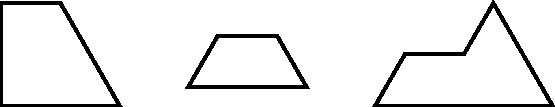
\includegraphics{rep-4-tile2.pdf}
\]
Working with a partner, show that each of these polygons is a rep-4-tile.
\end{problem}


\begin{problem}
Explain why every rectangle whose sides have ratio $1:\sqrt{n}$ is a
rep-$n$-tile.
\end{problem}

\begin{problem}
Explain how you know that any rep-tile will tessellate the plane.
\end{problem}

\begin{problem}
Give an example of a polygon that tessellates the plane that is not a
rep-tile.
\end{problem}


\begin{problem}
Every tessellation made by rep-tiles will have \index{symmetry of
scale}\textbf{symmetry of scale}. What does it mean to have \textit{symmetry of scale}?
\end{problem}

\begin{problem}
Consider the tessellations made by rep-tiles you've seen so far. What
other symmetries do they have?
\end{problem}

\begin{problem}
Do you think you can have a tessellation that has symmetry of scale
but no other symmetries?
\end{problem}
\end{document}
